\section{Tails Analysis}

At this point we should have notice that the real danger of investments does not resides solely within the standard concept of dispersion (standard deviation), nor within the ratio between return and dispersion. The true risk dwells in the worst case scenarios of the distributions, the tails. Where accumulated or great losses may strike down the whole investment plan. Hence, in order to address the risk analysis of any savings strategy, we need to take a closer look at the tails of their distributions.


Taking a close look at Figure \ref{fig:both_fw}, we are not able to clearly state which one is \textit{less risky}. So far, we have been comparing the values of Expected Shortfall in order to get a sense of the risk. But, since the ES is actually just the average of the tail of the distribution, we will now discuss how we can pursue a more in-depth analysis for the distribution of those tails.

In this section, we will go one step further and try to fit some specific distribution to those tails. This way we will be able to see in more detail the behaviour of the losses of our strategies, and set more accurate risk measures.

\subsection{Definition of \textit{Tail}}

First things first. What is \emph{the} Tail of a distribution? The tail of a distribution is not a precisely defined term; it can have many different forms and definitions. Generally, the \textit{tail} is considered a broad term to name the extreme parts of a distribution. In other words, there is not some specific place where you stop being in the middle of the distribution and start being in the tail, and where to put that line is up to every case.

Let's say that we plot a distribution $Y$, the loss of a savings plan (note that negative losses imply profits). We decide to put the distinction between middle and tail at some point named $u$, so the tail would be everything that lands within $Y>u$.

If we understand the tail of a distribution as a distribution itself, we can move that tail to the origin and normalise its area. Thus, being positively defined as

\begin{align}
    Z = \qty(Y-u | Y>u)
\end{align}.

Once we have this definition, we can easily define the probability density as

\begin{align}
    F_Z(z)  &=  P(Z < z) = P\qty(Y-u < z | Y>u)  \\
            &=  P\qty(Y<z+u | Y>u) \\
            &= \frac{P\qty(Y<z+u, Y>u)}{P\qty(Y>u)}
\end{align}

And thus, deriving this expression we find that, for every $z>0$,

\begin{align}
    f_z(z) = \frac{f_y\qty(z+u)}{1-F_y(u)}\textit{.}
\end{align}

Interesting thing about this result, is that we can analytically relate the distribution of the tail $f_z(z)$ with the whole original distribution $f_y(z)$.

Therefore, we can say that, if the distribution of the losses obtained is $Y$, our tail could be defined as

\begin{align}
    F_u(y) = \qty( Y - u \leq y| Y > u ) \emph{.}
\end{align}

The Pickands-Balkema-de Haan theorem states that for a large class of distributions $X$, exists $u$ such as that $F_u$ is well approximated by the Generalized Pareto Distribution (GPD). Where the standard cumulative distribution function of the GPD can be defined as:


\[F_{\xi}(y) = \left\{
  \begin{array}{lr}
    1 - \qty(1 + \xi \frac{y}{\psi})^{\sfrac{-1}{\xi}} & : \xi \neq 0\\
    1 - e^{-\sfrac{y}{\psi}} & : \xi = 0
  \end{array}
\right. \emph{.}
\]

Thus, we can seek that point $u$ from which our tail could fit a GPD. That would imply that, from that point $u$ forward, the distribution follows a GPD. The kind of GPD would be determined by the value of $\xi$. This number, usually called \emph{Extreme Value Index}, that determines  the shape of the distribution. The larger the value of $\xi$, the thicker the tail grows, and the slowly it converges to zero. In general:

\begin{itemize}
    \item $\xi > 0$. The tail does not converge to zero, ever. Power-law
    \item $\xi = 0$. The tail converges to zero at infinity. Exponential
    \item $\xi < 0$. The tail converges to zero in a finite point.
\end{itemize}

In what risk analysis concerns, the value of $\xi$ is crucial. Since we are studying the risk of a strategy looking at the tail of distributions where distribution are the frequency of losses, we could think that the wider or thicker the tail, the riskier the strategy.

\subsection{Extreme Value Analysis: Fitting a General Pareto Distribution}

Let us repeat the simulation for the CPPI, using $\pi = 0.1$, and plot the histogram of its losses as an example.

\begin{figure}[h]
    \centering
    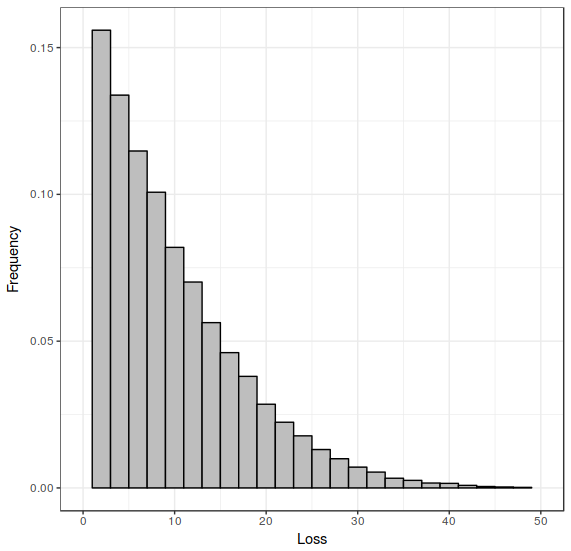
\includegraphics[scale=0.75]{images/cppi-losses-hist.png}
    \caption{Frequency Histogram of the losses of the CPPI strategy. Using $\pi = 0.1$, $\alpha = 0.0343$, $\sigma = 0.1544$ and $1000000$ simulations.}
    \label{fig:cppi-losses-histogram}
\end{figure}

If we now plot that density as points in a logarithmic scale, we might see something like the following:

\begin{figure}[h]
    \centering
    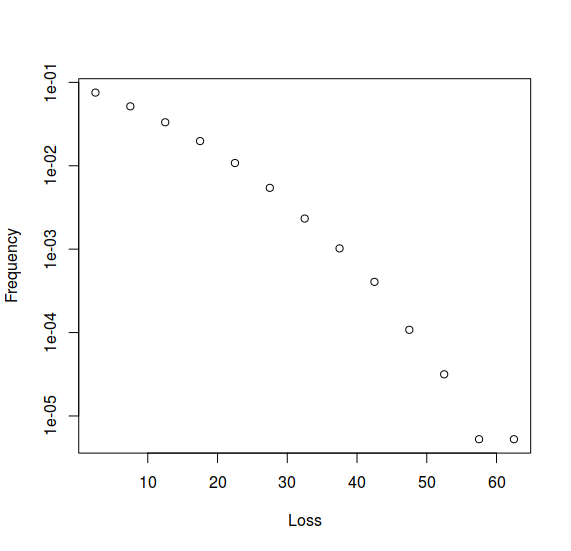
\includegraphics[scale=0.75]{images/cppi-dens-points.png}
    \caption{Density Distribution of the losses of the CPPI strategy in a logarithmic scale. Using $\pi = 0.1$, $\alpha = 0.0343$, $\sigma = 0.1544$ and $1000000$ simulations.}
    \label{fig:cppi-dens-points}
\end{figure}

Now, we could try to add here the Complementary Cumulative Distribution Function of a Generalized Pareto Distribution, and see if it fits to our distribution as it is now.

\begin{figure}[h]
    \centering
    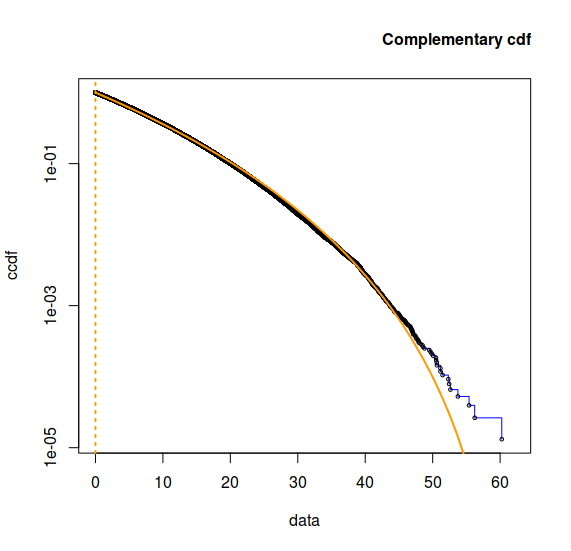
\includegraphics[scale=0.75]{images/cppi-ccdf-0.png}
    \caption{Density Distribution of the losses of the CPPI strategy in a logarithmic scale. Using $\pi = 0.1$, $\alpha = 0.0343$, $\sigma = 0.1544$ and $1000000$ simulations.}
    \label{fig:cppi-ccdf-0}
\end{figure}

Clearly, we can see how badly it fits for larger numbers. This indicates that our distribution is not following a GPD. Nevertheless, we can still find a proper $u$ for which it would.

A usual method in order to seek that $u$ threshold is to consecutively trying increasing numbers until one fits the distribution properly. We know that for that value on, the distribution will follow a GPD.

In this example, the first value that we find satisfies this is $u = 42.59$. And the result can be visualized in the following plot:

\begin{figure}[h]
    \centering
    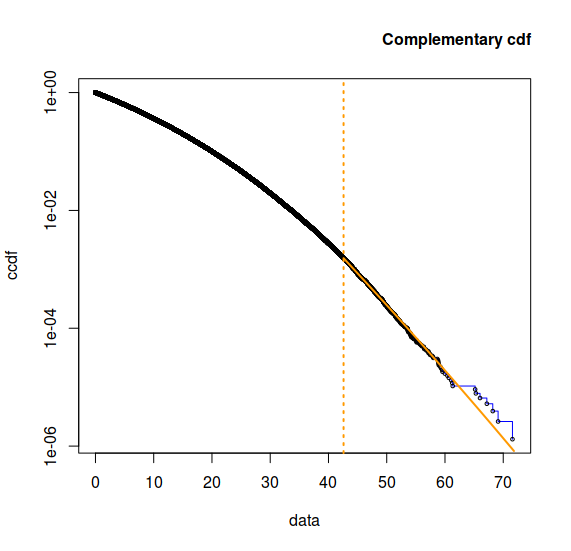
\includegraphics[scale=0.75]{images/cppi-ccdf-autothresh.png}
    \caption{Exploratory empirical residual coefficient of variation of losses of the CPPI strategy in a logarithmic scale. Using $\pi = 0.1$, $\alpha = 0.0343$, $\sigma = 0.1544$ and $1000000$ simulations.}
    \label{fig:cppi-ccdf-autothresh}
\end{figure}

The Extreme Value Index (EVI) obtained in this example is $\xi = 0.14$. This value of $\xi$ would suggest that the result of our model's distribution is of some kind with very fat tails, as a Power Law.

\subsection{Convergence of the Expected Shortfall}

So far, we have addressed the necessity of studying the tail of loss danger using the Expected Shortfall. It is quite straightforward and it easily assesses the risk of the tail. But since in order to get the Expetced Shortfall, what we are computing is the average of the tail of the distribution (in this case, marking the origin of the Tail as its VaR). In our example, we have found that the tail might be following a Power Law. The theoretical mean of a power-law distributed quantity $Y$ is, by defintion, given by

\begin{align}\label{eq:power-law-div}
\begin{split}
    \overline{Y} &= \int_{Y_{min}}^{\infty}Yp(Y)\dd{Y} =
    \pedra
    = \frac{C}{2 - \alpha}Y^{-\alpha + 2}\biggr\rvert_{Y_{min}}^{\infty}
\end{split}
\end{align}

It needs to be noted that this expression diverges for $\alpha \leq 2$. That means that for that values a Power Law has no finite mean. But what does it mean for a distribution not to having a finite mean? We can surely get the actual data and calculate their average. And as we will always get a finite number. Only if we had an infinite number of simulations/experiments we would get a mean that actually diverges.

Hence, if we were to repeat our finite experiment many times and calculate their mean for every repetition, the computed average of those many means should be - formally - divergent as well. Since we are actually capable of computing the mean, the consequence of the divergence found in Equation \ref{eq:power-law-div} is that these means may fluctuate a lot. We can say that the lack of convergence is indeed stating that the mean is not a well defined quantity, because it might vary enormously from one measurement to another. The formal divergence of $\overline{Y}$ is a red flag for us that should prevent us from computing empirical means, since they might not be reliable.

Since a Power Law can be expressed as a particular case of a Generalized Pareto Distribution, a general way of evaluating the convergence of the Expected Shortfall would be to fit a GPD to our distribution and compute their \emph{Extreme Value Index} $\xi$. And since we know that $\alpha = \frac{1}{\xi}$, we can say that for $\xi \geq \sfrac{1}{2}$, the Expected Shortfall does not converge.

\begin{figure}[h]
    \centering
    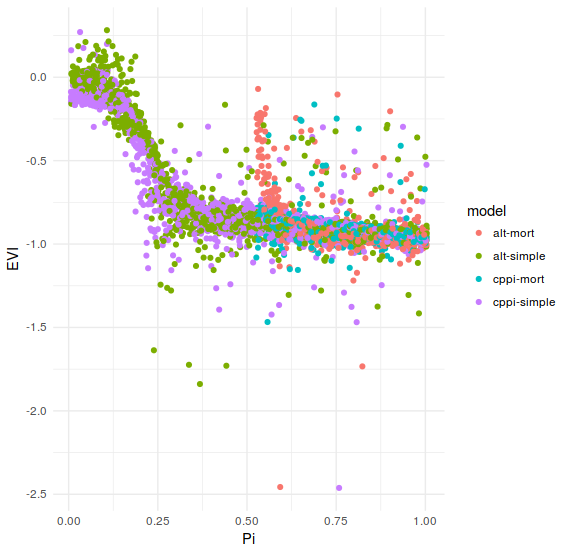
\includegraphics[scale=0.75]{images/evi-pi_.png}
    \caption{Extreme Value Index measured by varying values of $\pi$.  Using $\alpha = 0.0343$, $\sigma = 0.1544$, $A = 0.5$ and $1000000$ simulations.}
    \label{fig:evi-pi}
\end{figure}

In Figure \ref{fig:evi-pi} we can see a particular example in which none of the simulations happened to spot a situation where clearly $\xi \geq \sfrac{1}{2}$. Despite that, whereas for negatives values of $\xi$ we can fairly assume that the ES is going to converge, could not be the case for $\xi$ close to $0$ or even positive. In our results we have spotted some of the, specially in smaller values of $\pi$ got values so close to that critical value that we are not able to confirm that the ES might converge. This kind of result arises doubts on the reliability of some of the previously computed values for the Expected Shortfall.


\subsection{Extreme Value Index as Risk Measure}

In financial investment strategies and, in savings strategies, one of the main concerns is the assessment of risk. In order to address that, we make use of what we call \emph{risk measures}. We have discussed pros and cons of some of them. Is common practice to praise risk measures that falls withint the category of \emph{coherent risk measures}, and for good reasons, because gien a risk measure $\rho$, we define it as coherent if it satisfies the following properties:

\begin{align}
\begin{split}
    \rho(\lambda X) &= \lambda \rho (X) \\
    \rho(\lambda  + X) &= \lambda \rho(X) \\
    P(X_1 < X_2) &= 1 \implies \rho(X_1) < \rho(X_2) \\
    \rho(X_1 + X_2) &\leq \rho(X_1) + \rho(X_2) \emph{.}
\end{split}
\end{align}

Instead, the work of **INSERT REF** proposed the definition of Scale-free and Location-Free risk measures, defined by the following properties, where $X$ and $\rho$ are limited to be positive:

\begin{align}
\begin{split}
    \rho(\lambda X) &= \rho(X) \\
    \rho(\lambda + X) &= \rho(X) \\
    P(X_1 < X_2) &= 1 \implies \rho(X_1) < \rho(X_2) \\
    \rho(X_1 + X_2) &\leq \rho(X_1) + \rho(X_2) \emph{.}
\end{split}
\end{align}

We can see than the 1st and 2nd properties are different. Moreover, both the distribution and the risk measure are restricted to be positive. Whilst the latter seems reasonable and seamlessly interpretable, for the simplicity that comes avoiding "negative risk" results; the former might seem a bit odd at first. However, as we have discussed, is somehow misleading to consider the whole distribution in order to assess risk, because we might end pondering the probability of unusually huge benefits as a "risk", whereas limiting the distribution to the losses might be more reasonable. Thus, a distribution of the losses would fit the restrictions for this new kind of risk measure.

Moreover, in **INSERT REF** the authors propose the \emph{Extreme Value Index} as a Risk Measure. It surely satisfies the properties for a scale and location free risk measure, characterizes the worst case scenarios better than more standard measures as the \emph{VaR} or the \emph{Expected Shortfall}.

If the \emph{VaR} and the \emph{Expected Shortfall} gave us a sense of the location and scale of the worst scenario losses, the Extreme Value Index (EVI) can be interpreted as the thickness of the tail of the distribution. And this kind of assessment can be of great help, specially in those scenarios when the Expected Shortfall might not be reliable.

\begin{figure}[h]
    \centering
    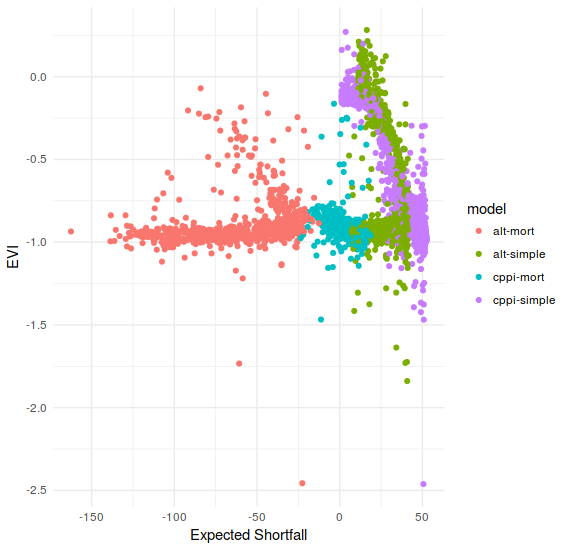
\includegraphics[scale=0.75]{images/evi-es_.png}
    \caption{Scatter plot of $10,000,000$ simulations of all four strategies, iterating over all values of $0 <= \pi <= 1$ and $0.5 <= A <= 2$ for the strategies without mortality and of $0.5 <= \pi <= 1$ and $0.5 <= A <= 2$ for the strategies with mortality.}
    \label{fig:evi-es}
\end{figure}

In Figure~\ref{fig:evi-es} it is shown that the relationship between the Expected Shortfall and the EVI is rather constant in most cases, except in those strategies that we know are more prone to greater losses, where the value of EVI increases considerably. This indicates that the EVI is not affected by the location and scale of the risk situation of each strategy, but indeed reflects the exposure to potential losses inherently present in some scenarios.



% \subsubsection*{Convergence of the Expected Shortfall}

% So far, we have addressed the necessity of studying the tail of loss danger using the Expected Shortfall. It is quite straightforward and it easily assesses the risk of the tail. But since it is nothing more than a simple mean, it can arise some issues.

% We talked about how the tail of a distribution can be considered a distribution by itself. Thus, the mean of the tail intends to be a summary statistic of this distribution. Despite that, we know that the arithmetic mean is not always a good summary statistic for every given distribution. There are some distributions from which the mean is not the best suited statistic to get a reliable feel of its \emph{general tendency}, especially on very skewed distributions.

% Moreover, without previous knowledge about the distribution we may encounter, it exists the possibility of facing a distribution whose arithmetic mean does not exist. This possibility arises a very disturbing problem: The computed value of the Expected Shortfall should not exist. Since we are working with simulated data, and thus finite numbers, we will never face an infinite arithmetic mean. This implies that in order to ensure the reliability of the Expected Shortfall, we first need to check whether its computation makes sense or not.

% In Figure \ref{fig:loss_both} we see the density curve of the loss tails of both methods. If we compute the histogram and set the bars of the histogram as points, we can build a scatterplot.
% In Figure \ref{fig:lm-tails} we can see this scatter plot of their logarithmic density points. It is of great interest noticing that, whereas both tails follow a linear model quite accurately (after taking logarithms), the \textit{Alternative} scheme has a much sharper descending trend. Which would mean that its \textit{Expected Shortfall} is far less likely to be infinite in any analytical distribution. This suggests us that the computed value of the Expected Shortfall is much more reliable for the \textit{Alternative} scheme than for the CPPI one.

% \begin{figure}[h]
%     \centering
%     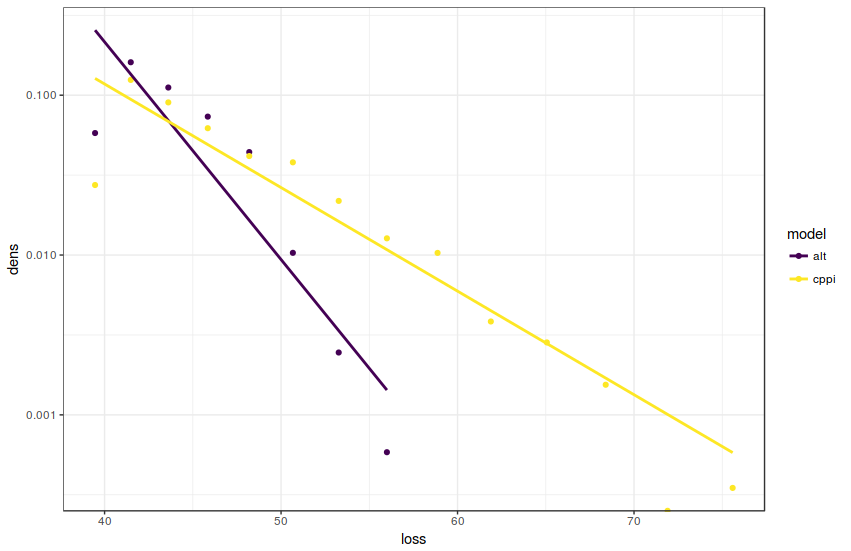
\includegraphics[scale=0.5]{images/lm_tails.png}
%     \caption{Scatter plot and linear regression of the logarithm of the density points of the \textit{CPPI} and \textit{Alternative} methods.}
%     \label{fig:lm-tails}
% \end{figure}

